\documentclass{beamer}

\usepackage[utf8]{inputenc}
\usepackage[french]{babel}
\usepackage[T1]{fontenc}
\usepackage{tikz}
\usetikzlibrary{shapes, arrows}

\usetheme{Montpellier}
\usecolortheme{lily}

\setbeamertemplate{caption}{\insertcaption} 
\setbeamertemplate{footline}[frame number]

\title{Projet SAR - Une interface graphique pour la logique}
\institute[\textsc{Université Pierre et Marie Curie}]{
\includegraphics[width=3cm]{logo.png}}
\author{Sandra \textsc{LADURANTI} et Bastien \textsc{RIGAULT}}
\date{}
\begin{document}


%SLIDE 1

\begin{frame}
%
\includegraphics[width=0.20\textwidth]{logo}
\titlepage	
\footnotesize
\begin{tabular}[t]{@{}l@{\hspace{3pt}}p{.3\textwidth}@{}}
\emph{Référents:} \\
Béatrice \textsc{BERARD}\\
Mathieu \textsc{JAUME}\\
Bénédicte \textsc{LEGASTELOIS}\\
\end{tabular}%
\end{frame}
	
%SLIDE 2
\section{Présentation du projet}
\begin{frame}
\frametitle{Présentation du projet}
\begin{center}
\textbf{Objectif :} Créer un outil graphique pour l'apprentissage de la logique du 1\ier ordre
\end{center}
\begin{itemize}
\setlength\itemsep{0.7cm}
\item Exemple de formule de la logique du 1\ier ordre :
\begin{center}
$\forall x (Rose(x) \Rightarrow estRouge(x))$
\end{center}
\item Contexte : Un jardin avec des fleurs
\item Vérification de formules sur un jardin grâce au moteur fourni en \textit{Python}
\end{itemize}
\end{frame}

%SLIDE DEMO
\section{Présentation du projet}
\subsection{Démonstration}
\begin{frame}
\begin{center}
Démonstration
\end{center}
\end{frame}

	
%SLIDE 3
\section{Architecture générale}
\begin{frame}
\frametitle{Architecture globale du projet}
\begin{center}
\begin{figure}[!h]
\includegraphics[scale=0.36]{vueGlobale.png}
\end{figure}
Outils principaux : \textit{Unity 5.0} et \textit{C\#}
\end{center}
\end{frame}

%SLIDE 4
\subsection{Définition de la grammaire pour la logique du 1\ier ordre}
\begin{frame}
\begin{center}
\frametitle{Définition inductive des formules du projet}
Définition inductive d'une formule $F$ :
\end{center}
\vspace{0.4cm}
$ F ::= P(x_1, x_2, ..., x_n) \ | \ \lnot F \ | \ F_1 \land F_2 \ | \ F_1 \lor F_2 \ | \ F_1 \Rightarrow F_2 \
| \ \forall x F \ | \ \exists x F $
\\
\vspace{0.2cm}
avec :
\setbeamertemplate{itemize items}[circle]
\begin{itemize}
\item $x_1, x_2, ..., x_n$: constantes ou variables
\item $P$: prédicat ($Rose, estRouge, estGrand, ...$)
\end{itemize}
\vspace{0.6cm}
\begin{tabular}{lll}
\raisebox{-.25\height}{
\includegraphics[scale=0.15]{greenTick.png}} & $\forall x (Rose(x) \Rightarrow estRouge(x))$
\end{tabular}
\\
\vspace{0.5cm}
\begin{tabular}{lll}
\raisebox{-.25\height}{
\includegraphics[scale=0.15]{redCross.jpg}} & $\forall x (Rose(x) \: estRouge(x))$
\end{tabular}

\end{frame}

%SLIDE 5
\section{Analyse syntaxique d'une formule}
\subsection{Utilisation du parseur généré avec Grammatica}
\begin{frame}
\frametitle{Analyse syntaxique}
\begin{center}
\begin{figure}[!h]
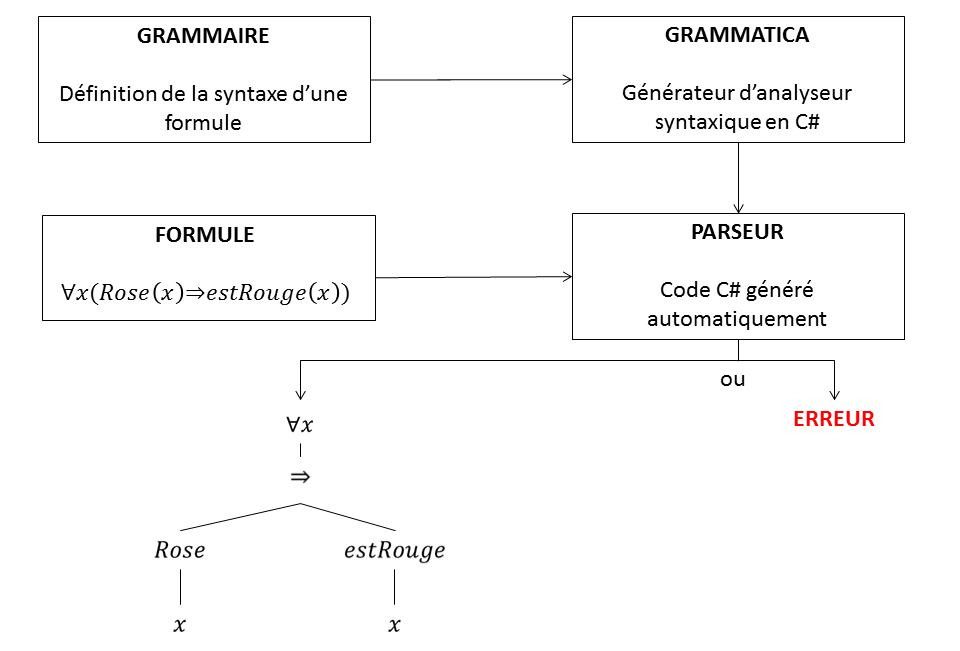
\includegraphics[scale=0.35]{syntaxTree.png}
\end{figure}
Outil utilisé : \textit{Grammatica 1.6}
\end{center}
\end{frame}



%SLIDE 6
\section{Vérification d'une formule}
\begin{frame}
\frametitle{Vérification d'une formule sur un jardin}
\begin{center}
\begin{figure}[!h]
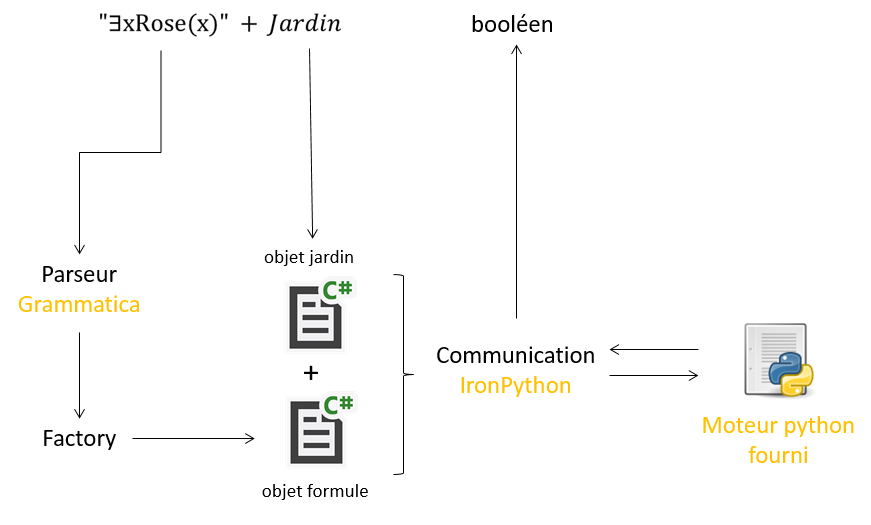
\includegraphics[scale=0.4]{verification.png}
\end{figure}
\end{center}
\end{frame}

%SLIDE 7
\section{Interface graphique}
\subsection{Aspect général}
\begin{frame}
\frametitle{Rendu final de l'application}
\begin{center}
\begin{figure}[!h]
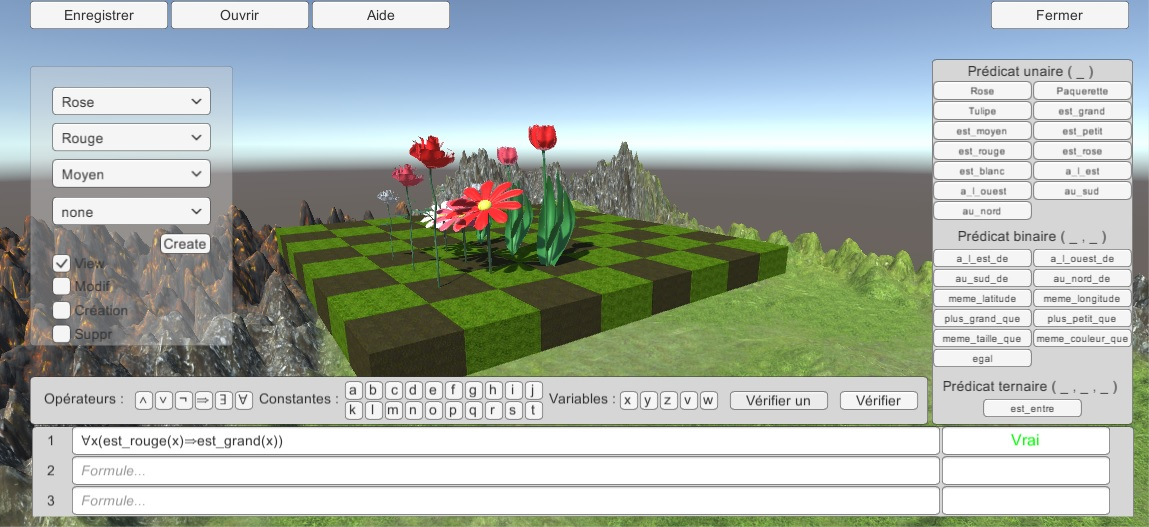
\includegraphics[scale=0.35]{renduFinal.jpg}
\end{figure}
\end{center}
\begin{itemize}
\item 4 éléments principaux : Le jardin, l'édition de formule, la création de fleurs et la barre d'outils
\item Programmation par scripts écrits en \textit{C\#}
\end{itemize}
\end{frame}

%SLIDE 8
\subsection{Création de fleurs dans le jardin}
\begin{frame}
\frametitle{Création de fleurs et édition du jardin}
\begin{center}
\begin{figure}[!h]
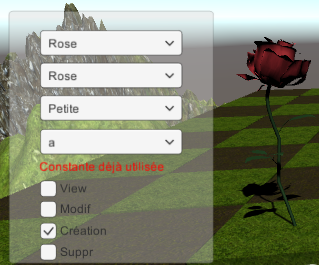
\includegraphics[scale=0.55]{creationFleur.png}
\end{figure}
\end{center}
\begin{itemize}
\setlength\itemsep{0.5cm}
\item Boucle principale d'execution
\item Génération et/ou suppression de fleurs
\end{itemize}
\end{frame}

%SLIDE 9
\subsection{Edition de formules}
\begin{frame}
\frametitle{Edition et vérification de formules}
\begin{center}
\begin{figure}[!h]
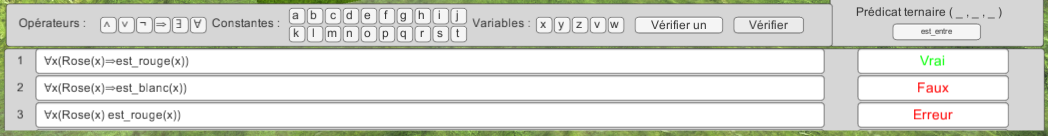
\includegraphics[scale=0.42]{clavier.png}
\end{figure}
\end{center}
\begin{itemize}
\setlength\itemsep{0.2cm}
\item Un bouton = Une chaîne de caractères à insérer dans un des formulaires
\item {
4 retours possibles :
\setbeamertemplate{itemize items}[circle]
\begin{itemize}
\item \textcolor{red}{Erreur} - la formule contient une erreur de syntaxe
\item \textcolor{orange}{VarLibre} - la formule contient une ou plusieurs variable(s) libre(s)
\item \textcolor{red}{Faux} - la formule n'est pas satisfaite par le jardin
\item \textcolor{green}{Vrai} - la formule est satisfaite par le jardin
\end{itemize}
}
\end{itemize}
\end{frame}


%SLIDE 10
\section{Problèmes rencontrés}
\begin{frame}
\frametitle{Problèmes rencontrés}
\begin{itemize}
\setlength\itemsep{0.5cm}
\item Problème de communication entre le moteur de vérification et \textit{C\#} au début du projet
\item Problème de coordination entre le clavier et les multiples formulaires
\item Problème de git au milieu de l'avancement du projet
\end{itemize}
\end{frame}

%SLIDE 11
\section{Conclusion}
\begin{frame}
\frametitle{Conclusion}
\begin{itemize}
\setlength\itemsep{0.5cm}
\item L'application finale est entièrement fonctionnelle
\item Le projet fut enrichissant de par son sujet et la variété d'outils mis en jeux pour sa réalisation
\item Des améliorations peuvent toujours être apportées (interface graphique plus ergonomique, nouvelles fonctionnalités...)
\end{itemize}
\begin{center}
Merci pour votre attention !
\end{center}
\end{frame}
	
\end{document}